\documentclass[a4paper,11pt,fleqn]{article}%fleqn pour aligner les equations à gauche
\usepackage{../../Styles/Cours}


\newcommand{\chnum}{Chapitre 12}
\newcommand{\chtitle}{Étude énergétique d'un mouvement}
\newcommand{\dtype}{TP}
 
  
\begin{document}
\maketitle

La tyrolienne est un mode de transport sur filin, permettant de se déplacer d'un point à un autre au-dessus du vide. Des installations de ce type sont fréquentes dans les parcours accrobranches en forêt mais se trouvent parfois dans des lieux plus insolites. En 2004, une tyrolienne a ainsi été installée entre le deuxième étage de la tour Eiffel et le Champ de Mars à ses pieds pour le passage de la flamme olympique en amont des Jeux d'Athènes. Une telle opération sera-t-elle reconduite en 2024 ?\\
\textbf{Dans cette activité, on se propose d'étudier une descente en tyrolienne d'un point de vue énergétique en s'intéressant plus particulièrement à l'évolution de l'énergie mécanique au cours de la descente.}
\begin{figure}[h!]
	\begin{minipage}{.6\textwidth}
	\begin{tcolorbox}[arc=1ex, colframe=black, left=3pt, right=3pt, top=3pt, bottom=2pt]
	\textbf{Échelle et angle de vue de la vidéo}\\
	La hauteur $h$ correspond à environ \SI{7}{\meter}. Cependant, l'angle de prise de vue de la vidéo, égal à \SI{45}{\degree}, fausse l'échelle verticale. On admet que cet effet peut être corrigé, pour une faible variation d'altitude, par : $y_1=1,41 y $
	\end{tcolorbox}
	\begin{tcolorbox}[arc=1ex, colframe=black, left=3pt, right=3pt, top=3pt, bottom=2pt]
	\textbf{Données :}
	\begin{itemize*}
		\item Masse de la personne sur la tyrolienne : $m =$ \SI{75}{\kilo \gram}
		\item Intensité de pesanteur : $q = $\SI{9,81}{\newton \per \kilo \gram}
		\item Hauteur du 2ème étage de la Tour Eiffel : \SI{115}{\meter}
	\end{itemize*}
	\end{tcolorbox}
	\end{minipage}
	\begin{minipage}{.4\textwidth}
	\begin{tcolorbox}[arc=1ex, colframe=black, left=3pt, right=3pt, top=3pt, bottom=2pt,height=6cm]
	
	\begin{center}
		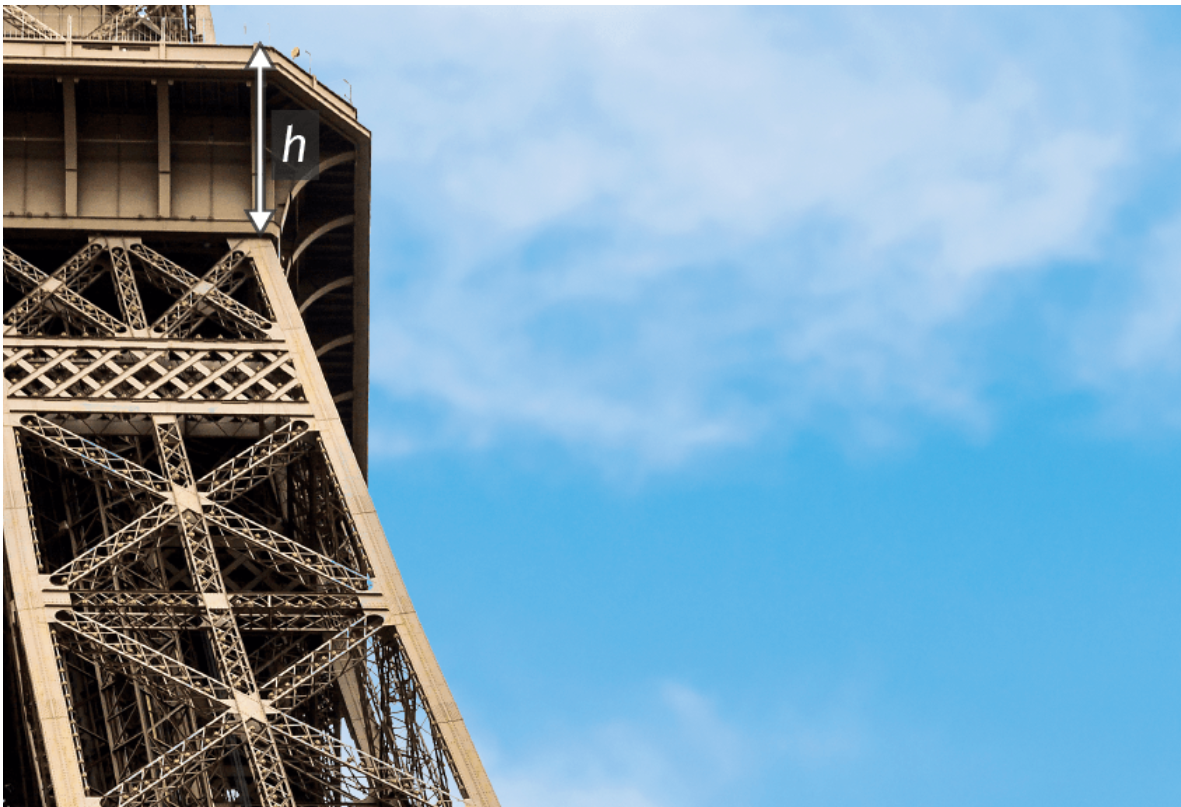
\includegraphics[scale=.17]{Ressources/TSPE_C5_Act3_Fig1.png}
	\end{center}
	\end{tcolorbox}	
	\end{minipage}
\end{figure}
\begin{enumerate}
	\item À partir de la vidéo de la descente en tyrolienne, réaliser le pointage du système, en plaçant l'origine du repère à la position initiale de la tyrolienne.
	\item Rappeler les expressions de l'énergie cinétique, de l'énergie potentielle de pesanteur et de l'énergie mécanique.
	\item Exploiter les données obtenues pour calculer, à chaque instant $t$, les grandeurs intermédiaires et finales mentionnées précédemment. (Attention : il faut créer au préalable la grandeur corrective $y_1$)
	\item Tracer sur un même graphique les courbes représentant l'évolution en fonction du temps de l'énergie cinétique, de l'énergie potentielle de pesanteur et de l'énergie mécanique.
	\item Interpréter (c'est-à-dire décrire et commenter) les courbes obtenues.
	\item Prévoir, en justifiant, l'évolution de l'énergie mécanique en fin de parcours.
\end{enumerate}
\textbf{Bilan :} Récapituler les étapes à suivre pour réaliser un pointage et faire l'étude énergétique d'un mouvement.\\
La descente visualisée ne correspond pas à la totalité de la descente réelle. Le reportage indique une vitesse finale de \SI{90}{\kilo \meter \per \hour}.
\begin{enumerate}[resume]
	\item En utilisant la conservation de l'énergie mécanique, déterminer la vitesse du système à son arrivée au sol si on considère le système en chute libre. Commenter.
\end{enumerate}
\end{document}